\subsection{M�todo Baseado em Entropia \label{entropia}}

Nascida na Termodin�mica, o conceito da Entropia � medir o grau de
desordem dos sistemas. Quanto maior for a desordem do sistema, maior
ser� a sua entropia, e uma imagem com entropia $0$ tem o mais baixo
n�vel de desordena��o.

Sendo $Pi$ a probabilidade da cor $i$ ocorrer nos pixels da imagem
$j$, a entropia $S$ � dada por :

\begin{large}
\begin{center}
\begin{equation}
\label{eq:entropia}
Sj = - \sum_{i=0}^{n}{Pi * ln(Pi)}
\end{equation}
\end{center}
\end{large}

A entropia m�xima se d� quando as cores estiverem desorganizadas,
quando a probabilidade de encontrarmos um pixel com uma dada cor �
igual para todas as possibilidades de cores.

Por exemplo : uma imagem em tons na escala de cinza, que tem uma
distribui��o igual para cada pixel, tem a probabilidade de
$\frac{1}{255}$ ($0,30$\%) de encontrarmos um pixel com o tom na
escala desejada. Esta imagem teria um histograma igual ao da Figura
\ref{img_entropia_maxima}

\begin{figure}[h|top]
 \centering
 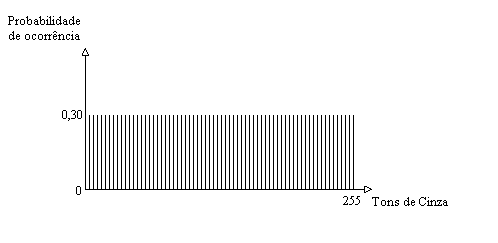
\includegraphics[width=0.6\linewidth]{imagens/entropia_maxima.png}
 \caption{Histograma de uma imagem com entropia M�xima.}
 \label{img_entropia_maxima}
\end{figure}

Com isso, a entropia m�xima $S$ � dada por:

\begin{large}
$ Sj = - ( \frac{1}{255} * \log{\frac{1}{255}} ) * 255 $

$ Sj = - ( 0,0039 *  -2,4065 ) * 255 $

$ Sj = - ( -2,4065 ) $

$ Sj = 2,4065 $

\end{large}

que � igual a :

\begin{large}
$ Sj = - \log{\frac{1}{255}} $

$ Sj = 2,4065 $

\end{large}

A entropia minima se da quando em todos os pixels existe somente uma
cor, como exemplo uma imagem em branco, logo a probabilidade de
encontrarmos uma cor � $100$\%. Esta imagem tem um histograma igual
ao da figura \ref{img_entropia_minima}.

\begin{figure}[h|top]
 \centering
 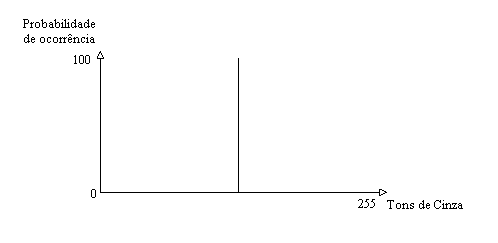
\includegraphics[width=0.6\linewidth]{imagens/entropia_minima.png}
 \caption{Histograma de uma imagem com entropia M�nima.}
 \label{img_entropia_minima}
\end{figure}

Com isso, a entropia m�nima $S$ � dada por:

\begin{large}
$ Sj = - ( 1 * \log{1} ) $

$ Sj = 0 $
\end{large}

Neste trabalho a entropia ser� aplicada como m�todo de
dissimilaridade entre os frames
